\chapter{Software Architecture Design}
\label{chap:software-architecture-design}

\section{System Architecture Overview}
\label{section:architecture-overview}

Figure~\ref{fig:system-architecture} shows the high-level system architecture.

\begin{figure}[H]
    \centering
    
\includegraphics[width=0.9\textwidth]{system-architecture.png}
    \caption{System architecture overview.}
    \label{fig:system-architecture}
\end{figure}

The system consists of five components:

\begin{itemize}
    \item \textbf{Web App (React).} The user-facing frontend. Users upload videos, enter search queries, browse face clusters, and view results through this interface. It communicates with the backend exclusively through HTTP requests.

    \item \textbf{REST API (FastAPI).} The central coordinator. It receives upload and search requests from the Web App, validates inputs, and routes them to the appropriate service. For uploads, it dispatches processing jobs to the Task Queue. For searches, it encodes the query through the AI Pipeline and runs similarity search against the Vector DB.

    \item \textbf{Task Queue (Celery + Redis).} Handles video processing asynchronously. When a video is uploaded, the REST API enqueues a processing job rather than blocking the user. The Task Queue picks up the job and runs the AI Pipeline in the background, allowing users to continue using the application while their video is being indexed.

    \item \textbf{AI Pipeline (SAM + SigLIP2 + InsightFace).} The core intelligence of the system. It operates in two modes: during ingestion, it segments objects (SAM), encodes regions and whole frames (SigLIP2), aggregates tracked object embeddings across frames (TAM), and detects faces (InsightFace). During search, it encodes the user's query into the same vector space for similarity matching.

    \item \textbf{Storage.} Split into two parts. The \textbf{Vector DB} (FAISS) stores all embeddings with metadata (timestamps, bounding boxes, source camera) and handles fast similarity search. \textbf{File Storage} holds the original video files for playback when users click on a search result.
\end{itemize}

Figure~\ref{fig:pipelines} zooms into the AI pipeline, showing its two operating modes.

\begin{figure}[H]
    \centering
    \begin{minipage}[c]{0.48\textwidth}
        \centering
        
\includegraphics[width=\textwidth,height=0.35\textheight,keepaspectratio]{ingestion-pipeline.png}
        \par\vspace{4pt}
        (a) Ingestion Pipeline
    \end{minipage}
    \hfill
    \begin{minipage}[c]{0.48\textwidth}
        \centering
        
\includegraphics[width=\textwidth,height=0.35\textheight,keepaspectratio]{search-pipeline.png}
        \par\vspace{4pt}
        (b) Search Pipeline
    \end{minipage}
    \caption{Detail of the AI pipeline from Figure~\ref{fig:system-architecture}.}
    \label{fig:pipelines}
\end{figure}

\textbf{(a) Ingestion Pipeline.} Uploaded video is split into keyframes at 1--5 FPS. Each frame goes through two parallel paths. SAM \cite{kirillov2023segment} segments every object in the frame into regions with context padding. SigLIP2 \cite{zhai2025siglip2} then encodes each region and the whole frame into 768-dimensional vectors. The Temporal Aggregation Module (TAM, see Section~\ref{subsubsec:tam}) merges embeddings of the same object tracked across frames into one representative vector, reducing index size and duplicate results. In parallel, InsightFace \cite{deng2019arcface} detects and encodes faces. All embeddings are stored with timestamps in the vector database.

\textbf{(b) Search Pipeline.} The user's text or image query is encoded by SigLIP2 into the same vector space. FAISS performs cosine similarity search against all stored embeddings. A hybrid scoring function then computes each image's final score as the maximum of its best region score and whole-image score, ensuring small objects detected by SAM are not lost. Results are ranked and returned with timestamps.

\section{Software Design}
\label{section:software-design}

This section describes the runtime behavior of the system through sequence diagrams for the two most important use cases.

\subsection{Video Upload and Indexing (UC-4)}

The following diagram shows the sequence of interactions when a user uploads a video.

\begin{figure}[H]
    \centering
    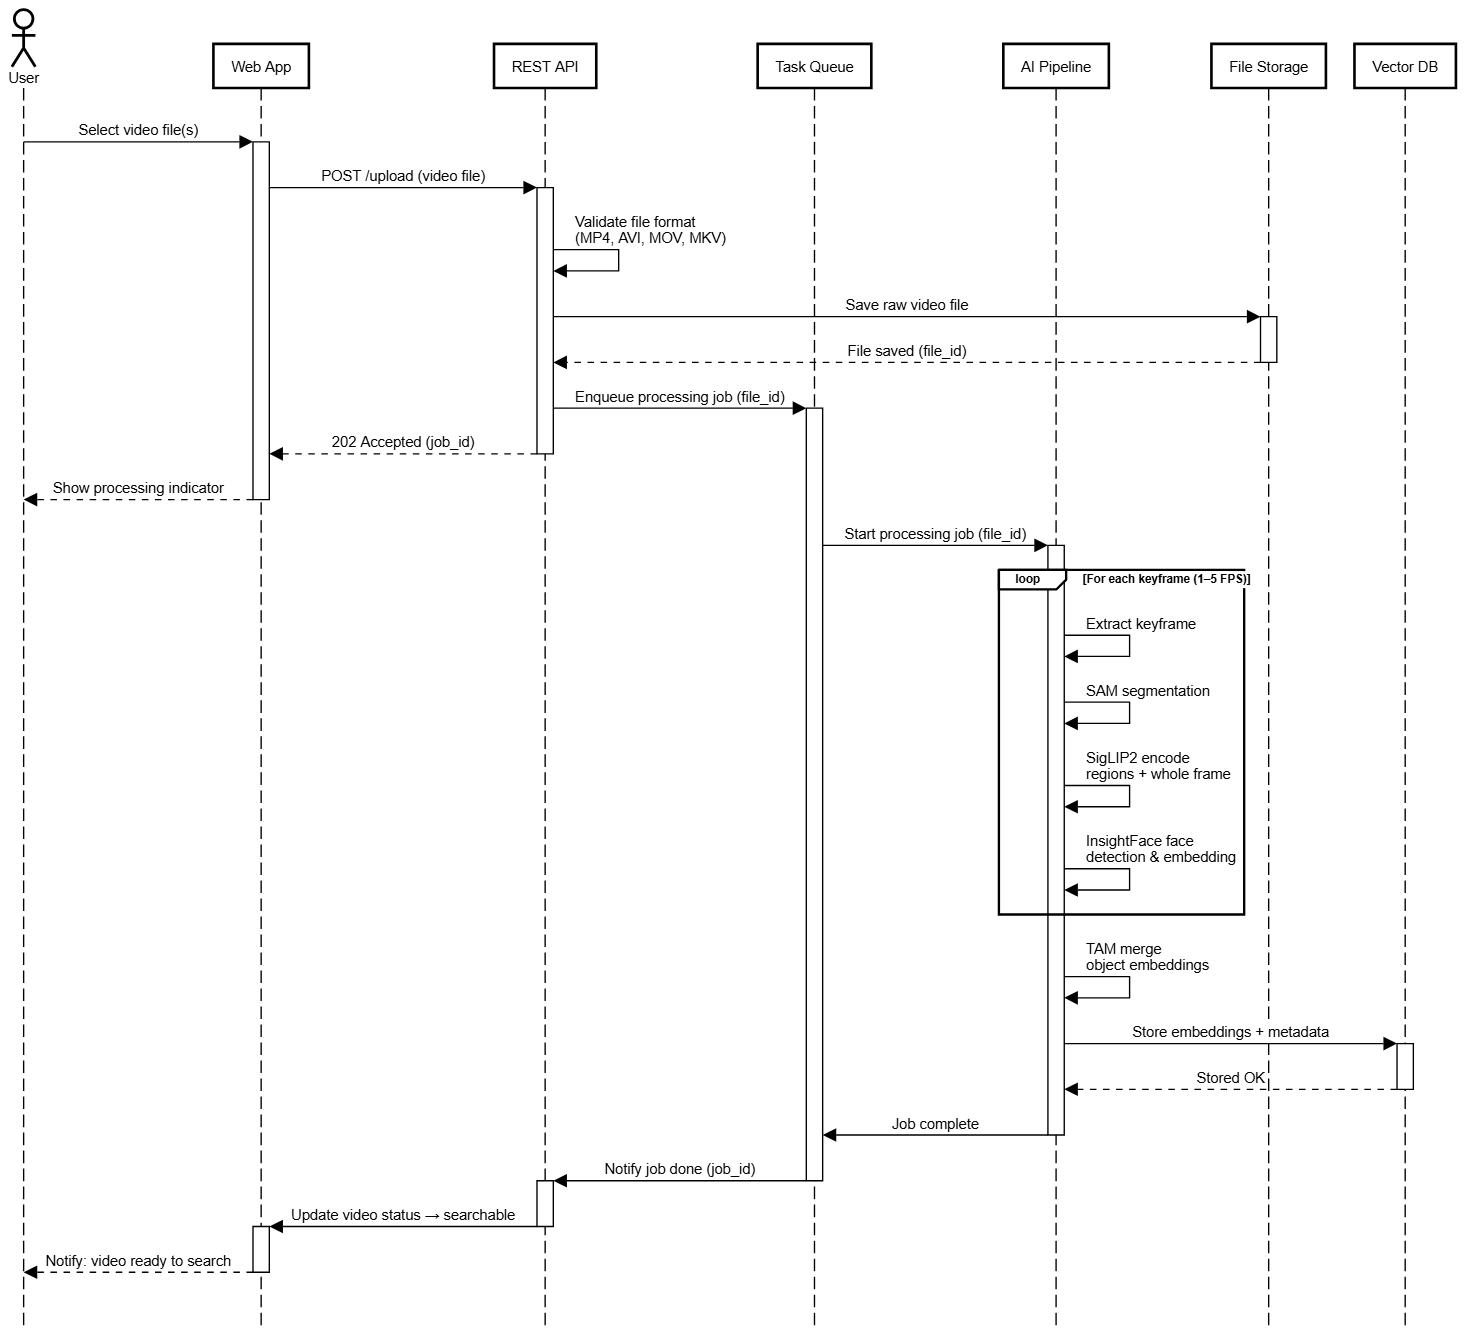
\includegraphics[width=0.85\textwidth]{assets/UC-4 - Sequence Diagram.png}
    \caption{Sequence diagram for video upload and indexing (UC-4).}
    \label{fig:seq-upload}
\end{figure}


\subsection{Text Search (UC-1)}

Figure~\ref{fig:seq-search} shows the sequence of interactions when a user performs a text search.

\begin{figure}[H]
    \centering
    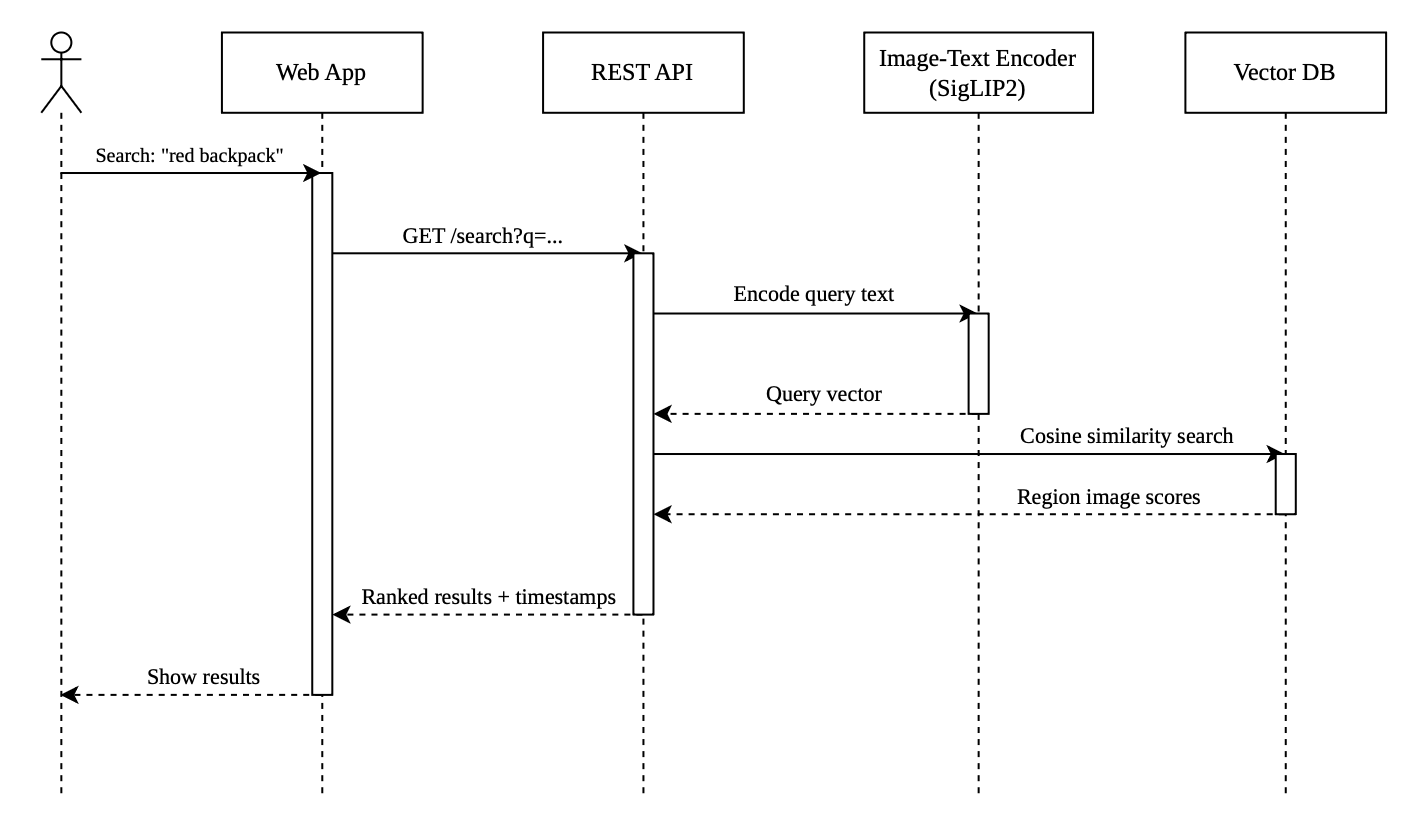
\includegraphics[width=0.85\textwidth]{assets/search-seq.png}
    \caption{Sequence diagram for text search.}
    \label{fig:seq-search}
\end{figure}

The user submits a text query through the Web App. The REST API sends the query to the AI Pipeline, where SigLIP2 encodes it into a 768-dimensional vector. The REST API then performs cosine similarity search against the Vector DB using FAISS. A hybrid scoring function computes each candidate's final score as the maximum of its best region score and whole-image score. The ranked results with timestamps are returned to the Web App for display.

\section{AI and Data Design}
\label{section:ai-data-design}

\subsection{Data Sources and Collection}

The system processes user-uploaded video footage as its primary data source. The following public datasets are used for development and evaluation:

\begin{itemize}
    \item \textbf{COCO val2017.} Image dataset with bounding box annotations across 80 object categories. Used for preliminary model selection and benchmarking.
    \item \textbf{UCA (UCF-Crime Annotation)} \cite{uca2024}. 23,542 sentence-level descriptions of surveillance video clips with temporal annotations. Used for training the Temporal Aggregation Module (see Section~\ref{subsubsec:tam}).
\end{itemize}

\subsection{Model Design}

The retrieval pipeline consists of two core components: a segmentation model and a vision-language encoder. To select the best combination, we conducted a preliminary benchmark on a subset of COCO val2017 (1,000 images, 66 queries across 5 categories). This benchmark is not the final system evaluation; it serves as a model selection experiment to inform our architecture decisions.

\subsubsection{Segmentation Model}

We use SAM (Segment Anything Model) \cite{kirillov2023segment} for class-agnostic segmentation. SAM segments every object in each frame without requiring a text prompt, which is essential for our offline indexing approach. Unlike text-prompted segmentation models such as Grounding DINO \cite{liu2023groundingdino} or OpenWorldSAM \cite{xiao2025openworldsam}, SAM does not need to know what the user will search for at indexing time. This allows the system to process footage once and handle arbitrary queries at search time.

\subsubsection{Vision-Language Encoder Selection}

We evaluated three vision-language encoders on whole-image retrieval to determine which produces the strongest embeddings. Table~\ref{tab:encoder-selection} summarizes the results.

\begin{table}[H]
    \centering
    \begin{tabular}{lccc}
        \toprule
        \textbf{Encoder} & \textbf{Recall@5} & \textbf{mAP} & \textbf{Small Obj. R@5} \\
        \midrule
        CLIP \cite{radford2021learning} & 0.570 & 0.376 & 0.244 \\
        BLIP \cite{li2019blip} & 0.036 & 0.014 & 0.022 \\
        \midrule
        \textbf{SigLIP2} \cite{zhai2025siglip2} & \textbf{0.703} & \textbf{0.537} & \textbf{0.411} \\
        \bottomrule
    \end{tabular}
    \caption{Vision-language encoder comparison on COCO val2017 (whole-image retrieval, 66 queries). SigLIP2 outperforms CLIP and BLIP across all metrics.}
    \label{tab:encoder-selection}
\end{table}

SigLIP2 achieves the highest scores on all metrics, making it the preferred encoder. However, all whole-image encoders struggle with small and background objects (rightmost column), motivating the addition of SAM segmentation.

\subsubsection{Effect of SAM Segmentation}

We then paired SAM with each encoder using our hybrid scoring approach, where the final score for each image is the maximum of the best region score and the whole-image score. Table~\ref{tab:sam-effect} shows the results.

\begin{table}[H]
    \centering
    \begin{tabular}{lccc}
        \toprule
        \textbf{Pipeline} & \textbf{Recall@5} & \textbf{mAP} & \textbf{Small Obj. R@5} \\
        \midrule
        SAM + CLIP & 0.654 & 0.407 & 0.519 \\
        \midrule
        \textbf{SAM + SigLIP2} & \textbf{0.748} & \textbf{0.549} & \textbf{0.619} \\
        \bottomrule
    \end{tabular}
    \caption{Effect of adding SAM segmentation. Both encoders improve, with SAM + SigLIP2 achieving the best results. Small object retrieval improves from 0.411 (SigLIP2 alone) to 0.619.}
    \label{tab:sam-effect}
\end{table}

Adding SAM segmentation improves both encoders, and the stronger encoder (SigLIP2) benefits more. Based on these results, we selected SAM + SigLIP2 as the retrieval backbone. The architecture is encoder-agnostic; the vision-language encoder can be swapped without changing the rest of the pipeline.

\subsubsection{Temporal Aggregation Module (TAM)}
\label{subsubsec:tam}

The region-level approach described above works well for static images, but video introduces a new challenge. When SAM tracks an object across consecutive frames, the same person walking through a 5-minute clip might appear in 300 frames, producing 300 near-identical embeddings in the index. This causes three problems: the index grows unnecessarily large, queries slow down, and search results are filled with duplicates of the same object.

The Temporal Aggregation Module (TAM) will solve this by merging multiple embeddings of the same tracked object into a single representative embedding. TAM is designed as a lightweight neural network that takes as input the N embeddings produced by SigLIP2 for one tracked object across N frames, along with the SAM confidence score for each frame. It will learn to assign higher weight to frames where the object is clearly visible and unoccluded, and lower weight to frames where the object is partially hidden, blurry, or at the edge of the frame. The output will be a single weighted-sum embedding that best represents the object, normalized for stable similarity search.

TAM will be trained on the UCA dataset \cite{uca2024}, which provides 23,542 sentence-level descriptions of surveillance video clips. The training objective is to produce embeddings that are as close as possible to the text description of the tracked object, so the module naturally learns to prefer frames where the object matches its description most clearly.

This module is the project's novel contribution. Existing work like SAM-CLIP Search \cite{mulani2025samclip} operates only on static images. TAM is what will extend region-based retrieval from images to video, making it practical for real surveillance footage where objects move, get occluded, and appear across hundreds of frames.

\subsection{Evaluation}

The system will be evaluated on two levels:

\begin{enumerate}
    \item \textbf{Retrieval quality.} Recall@1, Recall@5, Recall@10, Precision@5, and mAP on COCO val2017, comparing the full pipeline (SAM + SigLIP2) against whole-image baselines. Query categories include simple objects, attributed objects, relational queries, and small/background objects. Video retrieval with TAM is evaluated on UCA.
    \item \textbf{End-to-end system.} Query latency, indexing throughput (frames per second), and storage efficiency (embeddings per video minute). User testing with real surveillance footage to assess practical usability.
\end{enumerate}
